In the process of developing a machine learning model, 
various artifacts beyond source code are produced. An 
artifact refers to any file that serves as an input or 
output of a given process. In traditional software 
development, inputs such as source code and libraries 
qualify as artifacts, while outputs like object files 
and executables are also considered artifacts. For 
instance, in a build process, these outputs represent 
the results of transforming inputs through the 
compilation pipeline. \cite{wandb, pulicharla2024data}

In the context of machine learning, the most critical 
artifacts are datasets and models. Datasets act as the 
inputs to the training process, while models, which 
encapsulate learned parameters and structures, serve as 
the outputs of this process. \cite{pulicharla2024data}
\begin{figure}[H]
    \centering
    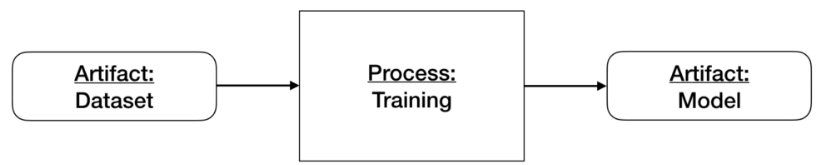
\includegraphics[width=0.8\textwidth]{fig/ml-artifacts.png}
    \caption{Artifacts in Machine Learning \cite{wandb}}
    \label{fig:ml-artifacts}
\end{figure}

\subsection{Use of Data Versioning in Machine Learning}

In machine learning workflows, managing datasets is as important 
as managing code, especially when it comes to reproducibility and 
collaboration. A systematic approach to data versioning enables 
teams to track, store, retrieve, and switch between different 
versions of datasets seamlessly, ensuring consistency across 
development and experimentation phases. \cite{wandb, pulicharla2024data}
\\\\
The process begins with versioning the dataset. Just as changes 
in source code are tracked, datasets need to be tracked too. 
Metadata files can be created to store information about each 
dataset version without including the actual dataset itself, 
keeping the repository efficient. These metadata files act as 
pointers to the specific dataset version associated with a 
particular stage of the machine learning pipeline. 
\cite{pulicharla2024data, opendatascience}
\\\\
Next, the dataset itself is stored in a dedicated storage 
system. This storage can be local or cloud-based, and it holds 
the actual data files. By separating the data from the metadata 
stored in the repository, teams can handle large datasets without 
bloating their version control systems, while still ensuring that 
every version is accounted for.\cite{opendatascience}
\\\\
Retrieving a specific dataset version is then made possible 
through the metadata file. The system can fetch the corresponding 
dataset version from storage based on the metadata, ensuring 
that the data matches the state of the code and experiments 
conducted at that time. This eliminates ambiguity and enhances 
reproducibility in experiments. \cite{opendatascience, yizhenzhao}
\\\\
Lastly, the ability to switch between dataset versions ensures 
flexibility during development. Just as a developer can revert 
to an earlier version of their code, they can also revert to or 
load the dataset version that was used with that code. This 
synchronization between code and data allows for iterative 
testing, analysis, and debugging, supporting more rigorous and 
reproducible experimentation. \cite{opendatascience, yizhenzhao}
\\\\
By implementing data versioning practices in this way, teams 
can ensure that their machine learning workflows are robust, 
efficient, and conducive to collaboration, enabling seamless 
transitions across different stages of development and research.
\cite{wandb, opendatascience, yizhenzhao}

\begin{figure}[H]
    \centering
    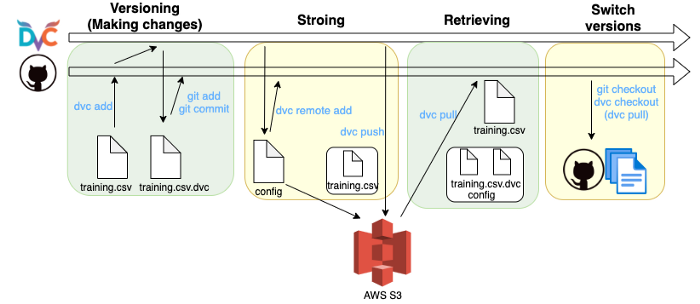
\includegraphics[width=0.8\textwidth]{fig/ml-dv-example.png}
    \caption{Example of how can be data versioning used in 
    machine learning (DVC and GIT as examples) \cite{opendatascience}}
    \label{fig:ml-dv-example}
\end{figure}

\subsection{Advantages of Data Versioning in Machine Learning}

In machine learning workflows, data versioning is not just 
about tracking changes; it also facilitates collaboration 
across multiple teams and ensures consistency in model 
development processes. By creating a structured system of 
versioning, practitioners can manage datasets and models at 
different stages of development, allowing seamless integration, 
testing, and improvement of machine learning pipelines.
\cite{wandb, opendatascience}
\\\\
Data versioning enables branching and merging of datasets, 
similar to how code branches work in software development. This 
is especially important when multiple teams or practitioners work 
on different aspects of a project. For instance, different projects 
or teams may use the same foundational dataset but modify or enhance 
it according to specific needs. These changes can be organized 
into separate "streams" or versions, ensuring that each team 
has a clear record of its modifications while still maintaining 
a connection to the original data.
\cite{wandb, opendatascience}
\\\\
Versioning also allows for "harvesting", where changes or 
improvements made in one branch can be integrated back into the 
main dataset or shared across other streams. This ensures that 
advancements in one area can benefit the broader workflow 
without disrupting other teams' progress. Similarly, the 
propagation of changes ensures consistency across different 
projects and keeps all streams aligned with the latest updates.
\cite{opendatascience, aimultiple}
\\\\
Moreover, data versioning systems can track multiple 
hierarchical streams, ranging from enterprise-level datasets 
to project-specific and even individual practitioners' 
workstreams. This hierarchical structure ensures flexibility 
and scalability, allowing datasets to evolve alongside their 
respective machine learning models.
\cite{opendatascience, aimultiple}
\\\\
By implementing a robust data versioning framework, teams can 
manage data lineage, collaborate effectively, and ensure 
reproducibility, even in complex machine learning ecosystems. 
This structured approach enhances the ability to build, test, 
and deploy models with greater confidence.
\cite{opendatascience, aimultiple}

\begin{figure}[H]
    \centering
    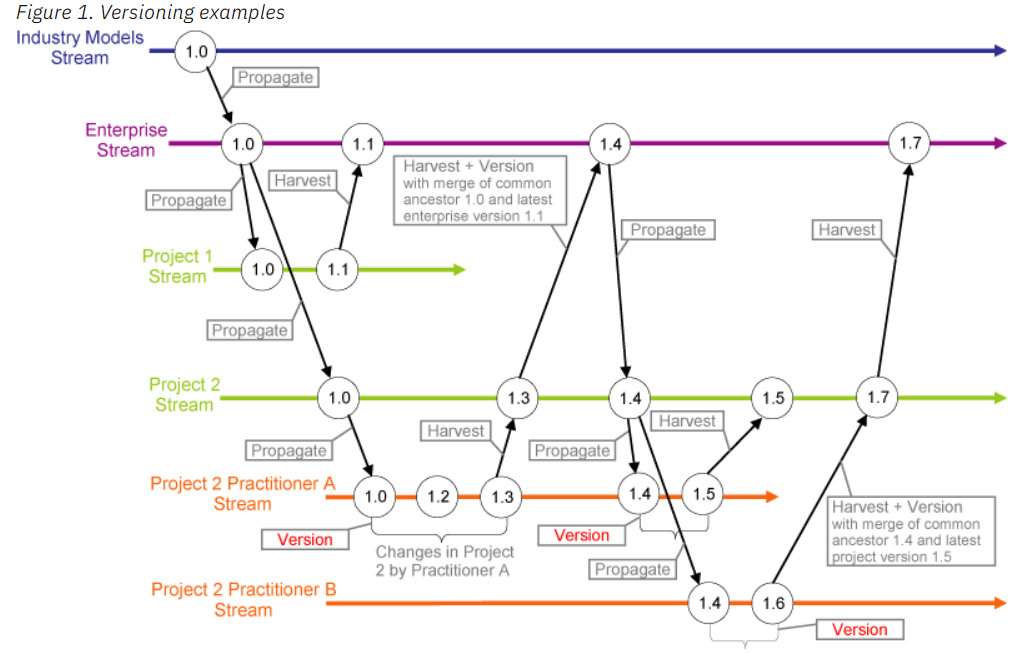
\includegraphics[width=0.8\textwidth]{fig/dv-advantages.png}
    \caption{An example of hierarchical data versioning 
        streams showcasing branching, propagation, and 
        merging across industry, enterprise, project, and 
        individual practitioner levels, enabling collaborative 
        and scalable data management in machine learning 
        workflows \cite{aimultiple}}
    \label{fig:dv-advantages}
\end{figure}
